\icode{E-MD-MU-L3-261120-002}
（多选）
如图所示，倾角为\(\alpha =\)\,\qty{37}{\degree}的斜面体静置在粗糙水平地面上，劲度系数为\(k\)的轻弹簧下端拴接在斜面体	底端的挡板上，质量为\(m\)的物块\(a\)拴接在轻弹簧的上端，放在斜面体上质量为\(m\)的物块\(b\)通过跨过光滑定滑轮的细绳与质量为\(2m\)的球\(c\)拴接。初始时\(a\)、\(b\)接触，\(c\)在外力的作用下，使\(b\)、\(c\)间绳子伸直但无拉力。物块\(b\)、滑轮间的细绳与斜面平行，斜面光滑，重力加速度为\(g\).撤去球\(c\)的外力一瞬间，下列说法正确的是\paren[]

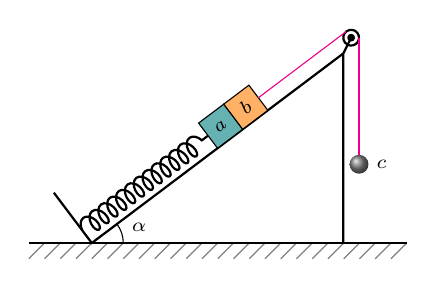
\begin{tikzpicture}[font=\scriptsize]
	\begin{scope}[rotate=37]
		\coordinate (P) at(4.28,.04);
		\draw[thick] (0,.8)--(0,0)--(4,0)--++(-127:2.4) (4,0)--(4.2,.1) (4.2,.1) circle(.1);
		\fill (4.2,.1) circle(.05);
		\draw[thick,decoration={aspect=.6,segment length=4,amplitude=1.2mm,coil},decorate] (0,.2)--(2,.2);
		\draw[fill=teal!60] (2,0) rectangle(2.4,.4)node[midway,rotate=37]{\(a\)};
		\draw[fill=orange!60] (2.4,0) rectangle(2.8,0.4)node[midway,rotate=37]{\(b\)};
		\draw[magenta] (2.8,.2)--(4.2,.2);
	\end{scope}
	\foreach \x in {-.8,-.6,...,3.8}
	\draw[gray] (\x,-.2)--++(.2,.2);
	\draw[thick] (-.8,0)--(4,0);
	\draw (.4,0) arc(0:37:.4);
	\draw[magenta] (P)--(P|-3,1);
	\shade[ball color=gray] (P|-3,1) circle(.12);
	\node[xshift=.1cm] at(P|-3,1)[right]{\(c\)};
	\node at(.6,.2){\(\alpha\)};
\end{tikzpicture}
\begin{choices}
	\item 物块\(b\)的加速度为\(2g\)
	\item 物块\(a\)的加速度\(0.5g\)
	\item 斜面体受到水平向右的静摩擦力作用
	\item 撤去球\(c\)的外力后，当弹簧弹力大小为\(\frac{15}{16}mg\)时，\(a\)、\(b\)刚好分离
\end{choices}
\begin{answer}
	BCD\qquad 提示：
\end{answer}